\documentclass[a4paper,11pt]{article}
\usepackage[utf8]{inputenc}
\usepackage{amsmath}
\usepackage{amsfonts}
\usepackage{amssymb}
\usepackage{graphicx}
\usepackage{braket}

\numberwithin{equation}{section}
\renewcommand\thesubsection{\alph{subsection}}
\newcommand{\bvp}[1]{\mathbf{#1}'}
\newcommand{\bv}[1]{\mathbf{#1}}
\newcommand{\ez}{\epsilon_0}
\newcommand{\eo}{\epsilon_1}
\newcommand{\lrp}[1]{\left({#1}\right)}
\newcommand{\lrb}[1]{\left\{{#1}\right\}}


%opening
\title{Electromagnetic Theory II HW3}
\author{Vince Baker}

\begin{document}

\maketitle

\section*{6.11}
a) The electromagnetic wave has momentum $\bv{g} = \bv{S}/c^2$ which is completely transferred to the absorbing medium. 
The momentum in the wave is constant in time, leading to a force of $\bv{F} = \bv{g}c\ dt = \bv{S}\ dt/c$.
Since the Poynting vector $\bv{S}$ is the energy per unit area of the wave, $\bv{S}\ dt/c$ is the energy in a differential volume element of the wave.\\
b) The acceleration due to the radiation pressure is $4.7x10^{-3}$ meters per second. 
To calculate the acceleration from the corpuscular radiation we need an estimate for the number and momentem of particles incident on $1 m^2$ of area.
One estimate puts the mean proton velocity at $700\ km/s$ and the proton density at $3.4\ cm^{-3}$ or $3.4\times 10^6\ m^{-3}$.
With a proton mass of $1.67\times 10^{-27}\ kg$ the total force due to the corpuscular radiation is $3.97\times 10^{-12}\ m/s$, a factor of $10^{11}$ less than the radiation pressure.

\section*{7.1}
We first invert the Stokes parameters for linear polarization (Jackson 7.27) to express the magnitudes and phase difference of the two linear polarization basis fields:
\begin{align}
 |\bv{E}_1| &= \sqrt{\frac{s_0+s_1}{2}}\\
 |\bv{E}_2| &= \sqrt{\frac{s_0-s_1}{2}}\\
 \delta_2-\delta_1 &= \cos^{-1}{\lrp{\frac{s_2}{\sqrt{s_0^2-s_1^2}}}}
\end{align}
We then invert the Stokes parameters in the circular polarization basis (Jackson 7.28):
\begin{align}
 |\bv{E}_+| &= \sqrt{\frac{s_0+s_3}{2}}\\
 |\bv{E}_-| &= \sqrt{\frac{s_0-s_3}{2}}\\
 \delta_--\delta_+ &= \cos^{-1}{\lrp{\frac{s_2}{\sqrt{s_0^2-s_3^2}}}}
\end{align}
We can now solve the electric field intensities.
a) In the linear polarization basis:
\begin{align}
 |\bv{E}_1| &= 1\\
 |\bv{E}_2| &= \sqrt{2}\\
 \delta_2-\delta_1 &= 45
\end{align}
In the circular polarization basis:
\begin{align}
 |\bv{E}_+| &= \sqrt{1/2}\\
 |\bv{E}_-| &= \sqrt{5/2}\\
 \delta_--\delta_+ &= 26.5
\end{align}
We plot the two time-varying fields against each other in MATLAB, with the (arbitrary) absolute phase of E1 equal to 0.
\begin{figure}[p]
 \caption{Signal polarization}
 \centering
   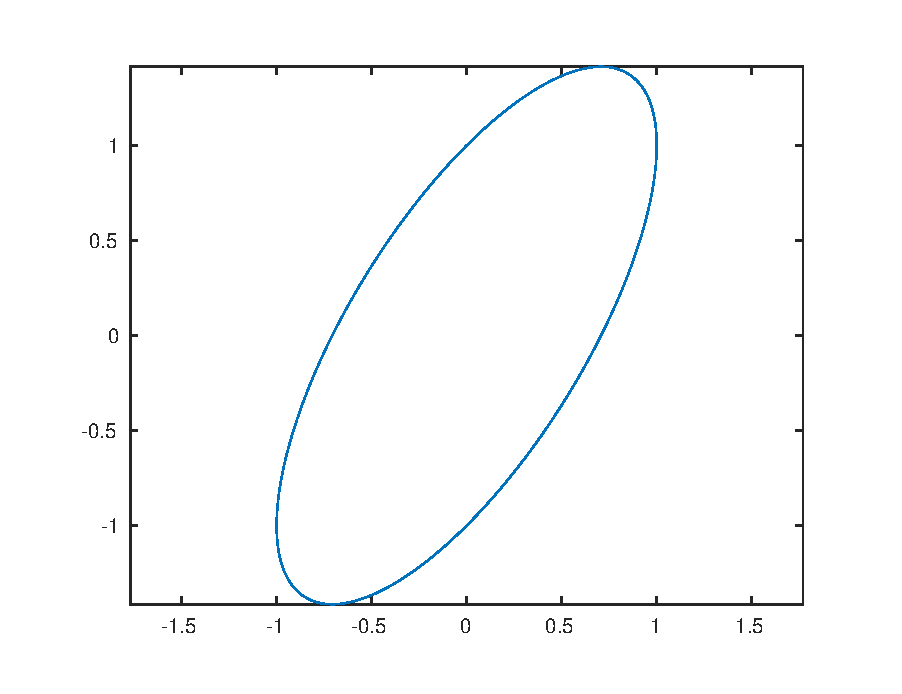
\includegraphics[width=\textwidth]{p71a}
\end{figure}
\\
b) In the linear polarization basis:
\begin{align}
 |\bv{E}_1| &= \sqrt{25/2}\\
 |\bv{E}_2| &= \sqrt{25/2}\\
 \delta_2-\delta_1 &= 16.2
\end{align}
In the circular polarization basis:
\begin{align}
 |\bv{E}_+| &= 4\\
 |\bv{E}_-| &= 3\\
 \delta_--\delta_+ &= 0
\end{align}
We plot the two time-varying fields against each other in MATLAB, with the (arbitrary) absolute phase of E1 equal to 0.
\begin{figure}[p]
 \caption{Signal polarization}
 \centering
   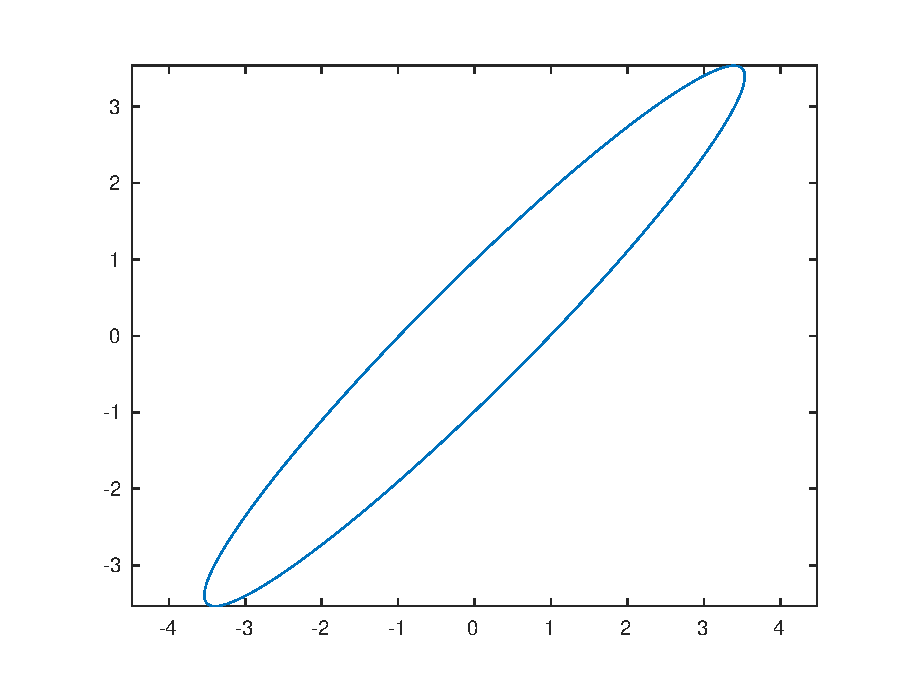
\includegraphics[width=\textwidth]{p71b}
\end{figure}

\section*{7.3}
a) The problem includes five different waves: the incident and reflected wave in the first region, the transmitted and reflected wave in the gap, and the transmitted wave in the second region.
With multiple regions there will be multiple reflections/transmissions, but the wave vectors of the different multiply-reflected components will be the same due to kinematic considerations and boundary conditions.
We will therefore solve the problem by first determining the kinematic part of the solution, then solving for the boudnary conditions as usual without any special consideration of the multiple reflections.
\\
We'll label the incident and reflected waves in the first section as $E_{1t}$ and $E_{1r}$, the transmitted and reflected waves in the gap as $E_{gt}$ and $E_{gr}$ and the transmitted wave in region 2 as $E_{2t}$.
Working the plane of incidence and applying Snell's law we have:
\begin{align}
 \theta_{1i} &= \theta_{1r} \equiv \theta_i\\
 n\sin{\theta_i} &= \sin{\theta_{gi}}\\
 \cos{\theta_{gi}} &= \sqrt{1-n^2\sin^2{\theta_i}}\\
 \theta_{gr} &= \theta_{gi}\\
 n\sin{\theta_{2t}} &= \sin{\theta_{gi}} = n\sin{\theta_i}\\
 \theta_{2t} &= \theta{i}
\end{align}

To maintain a consistent solution on the boundary the wave phases at the boundary must all be the same, and we set the phase to zero at $t=0$ and $z=0$.
The wave at the second boundary will have a phase offset $kd \sqrt{1-n^2\sin^2{\theta_i}}$. \\
We can now set up the boundary conditions for the case when the polarization is perpendicular to the plane of incidence.
We simplify the notation by defining $\gamma \equiv \sqrt{1-n^2\sin^2{\theta_i}},\ \phi \equiv kd\gamma$.
\begin{align}
 E_{1t}+E_{1i} &= E_{gt}+E_{gr}\\
 E_{gt}e^{i\phi}+E_{gr}e^{-i\phi} &= E_{2t}\\
 n(E_{1t}-E_{1r})\cos{\theta_{i}} &= (E_{gt}-E_{gr})\gamma\\
 (E_{gt}e^{i\phi}-E_{gr}e^{-i\phi})\gamma &= nE_{2t}\cos{\theta_i}
\end{align}
We can combine the first and third equations, eliminate one each of $E_{1t}$ and $E_{1i}$, and get:
\begin{align}
 E_{gt} &= \frac{1}{2}\lrp{E_{1i}(1+\frac{n\cos{\theta_i}}{\gamma})+E_{1r}(1-\frac{n\cos{\theta_i}}{\gamma})}\\
 E_{gr} &= \frac{1}{2}\lrp{E_{1i}(1-\frac{n\cos{\theta_i}}{\gamma})+E_{1r}(1+\frac{n\cos{\theta_i}}{\gamma})}
\end{align}
We can solve the second and fourth equations at the second boundary:
\begin{align}
 E_{gt} &= \frac{1}{2}e^{-i\phi}E_{2t}\lrp{1+\frac{n\cos{\theta_i}}{\gamma}}\\
 E_{gr} &= \frac{1}{2}e^{i\phi}E_{2t}\lrp{1-\frac{n\cos{\theta_i}}{\gamma}}
\end{align}
Setting the equations for $E_{gt}$ and $E_{gr}$ at the two boundaries equal to each other we can solve for the desired ratios:
\begin{align}
 \frac{E_{2t}}{E_{1i}} &= \frac{4\eta}{(1+\eta)^2e^{-i\phi}-(1-\eta)^2e^{i\phi}}\\
 \frac{E_{1r}}{E_{1i}} &= \frac{(1-\eta)^2(e^{i\phi}-e^{-i\phi})}{(1+\eta)^2e^{-i\phi}-(1-\eta)^2e^{i\phi}}
\end{align}
Where we have defined $\eta \equiv \frac{n\cos{\theta_i}}{\gamma}$.
\\
\\
The boundary conditions for the case when the polarization is parallel to the plane of incidence:
\begin{align}
 (E_{1t}-E_{1r})\cos{\theta_i} &= (E_{gt}-E_{gr})\sqrt{1-n^2\sin^2{\theta_i}}\\
 (E_{gt}e^{i\phi}-E_{gr}e^{-i\phi})\sqrt{1-n^2\sin^2{\theta_i}} &= E_{2t}\cos{\theta_i}\\
 n(E_{1t}+E_{1r}) &= E_{gt}+E_{gr}\\
 E_{gt}e^{i\phi}-E_{gr}e^{-i\phi} &= nE_{2t}
\end{align}
We again solve for $E_{gt}$ and $E_{gr}$ at the two boundaries and then equate them.
\begin{align}
 E_{gt} &= \frac{n}{2}\lrp{E_{1i}(1+\nu)+E_{1r}(1-\nu)}\\
 E_{gr} &= \frac{n}{2}\lrp{E_{1i}(1-\nu)+E_{1r}(1+\nu)}\\
 E_{gt} &= \frac{n}{2}e^{-i\phi}E_{2t}(1+\nu)\\
 E_{gr} &= \frac{n}{2}e^{i\phi}E_{2t}(1-\nu)
\end{align}
With $\nu \equiv \frac{\cos{\theta_i}}{n\gamma}$.
These have the same form as the equations for the perpendicular polarization (except for the factor of n, which cancels when combining them).
Therefore the transmitted and reflected ratios are:
\begin{align}
 \frac{E_{2t}}{E_{1i}} &= \frac{4\nu}{(1+\nu)^2e^{-i\phi}-(1-\nu)^2e^{i\phi}}\\
 \frac{E_{1r}}{E_{1i}} &= \frac{(1-\nu)^2(e^{i\phi}-e^{-i\phi})}{(1+\nu)^2e^{-i\phi}-(1-\nu)^2e^{i\phi}}
\end{align}
\\
b) The critical angle for total internal reflection is defined by $\sin^2{\theta_i} \ge 1/n^2$.

\end{document}
